% !TEX root = ../thesis.tex
\begin{figure}[h]
  \begin{center}
    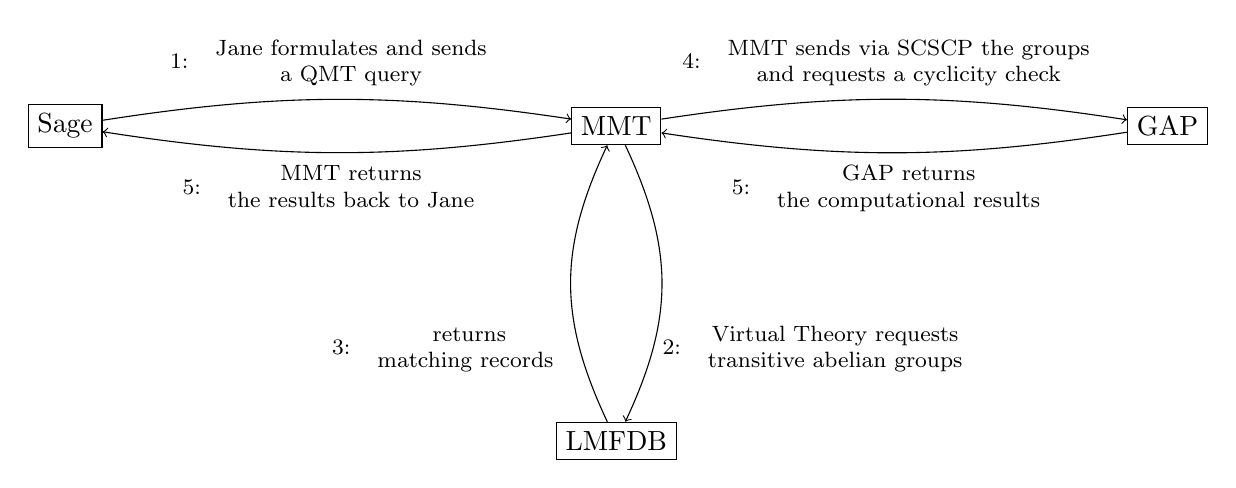
\begin{tikzpicture}[xscale=7,yscale=4]\normalsize
      \node[draw] (s) at (0,0) {Sage};
      \node[draw] (m) at (1,0) {MMT};
      \node[draw] (g) at (2,0) {GAP};
      \node[draw] (l) at (1,-1) {LMFDB};
      \draw[->] (s) to[bend left=15] node[above] {
        \footnotesize 1: 
        \begin{tabular}{c}
          Jane formulates and sends\\
          a QMT query
        \end{tabular}
      } (m);
      \draw[->] (m) to[bend left=15] node[right,near end] {
        \footnotesize 2: 
        \begin{tabular}{c}
          Virtual Theory requests \\
          transitive abelian groups
        \end{tabular}
      } (l);
      \draw[<-] (m) to[bend right=15] node[left,near end] {
        \footnotesize 3: 
        \begin{tabular}{c}
          \lmfdb\ returns\\
          matching records
        \end{tabular}
      } (l);
      \draw[->] (m) to[bend left=15] node[above] {
        \footnotesize 4: 
        \begin{tabular}{c}
          MMT sends via SCSCP the groups\\
          and requests a cyclicity check
        \end{tabular}
      } (g);
      \draw[<-] (m) to[bend right=15] node[below] {
        \footnotesize 5: 
        \begin{tabular}{c}
          GAP returns\\
          the computational results
        \end{tabular}
      } (g);
      \draw[<-] (s) to[bend right=15] node[below] {
        \footnotesize 5: 
        \begin{tabular}{c}
          MMT returns\\
          the results back to Jane
        \end{tabular}
      } (m);
    \end{tikzpicture}
  \end{center}

  \caption[A MiTM use-case]{
    Solving Jane's example of Cross-System Communication using our approach. 
  }
  \label{fig:mitmcaseintro}
\end{figure}